%==============================================================================
% Sjabloon poster bachproef
%==============================================================================
% Gebaseerd op document class `a0poster' door Gerlinde Kettl en Matthias Weiser
% Aangepast voor gebruik aan HOGENT door Jens Buysse en Bert Van Vreckem

\documentclass[a0,portrait]{hogent-poster}

% Info over de opleiding
\course{Bachelorproef}
\studyprogramme{toegepaste informatica}
\academicyear{2022-2023}
\institution{Hogeschool Gent, Valentin Vaerwyckweg 1, 9000 Gent}

% Info over de bachelorproef
\title{De kwetsbaarheden van een IPv6-
    netwerk en de mitigatie ervan in
    bedrijven.}
\subtitle{}
\author{Lander De Ghein}
\email{lander.deghein@student.hogent.be}
\supervisor{Karine Van Driessche}
\cosupervisor{Jochen Boutens (360IT)}

% Indien ingevuld, wordt deze informatie toegevoegd aan het einde van de
% abstract. Zet in commentaar als je dit niet wilt.
\specialisation{Systeem- en Netwerkbeheer}
\keywords{IPv6, Veiligheid, kwetsbaarheden}
\projectrepo{https://github.com/landerdg123/BPLanderDeGhein}

\begin{document}

\maketitle

\begin{abstract}

De opkomst van IPv6 brengt nieuwe cybersecurity-uitdagingen met zich mee, vooral voor kleinschalige bedrijven met beperkte middelen. Onderzoek naar IPv6-aanvallen is essentieel om effectieve beveiligingsmaatregelen te ontwikkelen. Het doel is inzicht te krijgen in de schadelijke gevolgen van aanvallen en optimale mitigatiemethoden te identificeren, met nadruk op het gebruik van opensource tools. Het streven is om de meest effectieve strategieën te ontdekken om IPv6-aanvallen te voorkomen, detecteren en beperken.
\end{abstract}

\begin{multicols}{2} % This is how many columns your poster will be broken into, a portrait poster is generally split into 2 columns

\section{Introductie}
IPv6 is de opvolger van het huidige IPv4-protocol dat wordt gebruikt voor internetcommunicatie. Hoewel IPv6 efficiënter en schaalbaarder is, brengt het ook nieuwe beveiligingsuitdagingen met zich mee. Om de beveiliging van IPv6 te waarborgen, is onderzoek essentieel.

Met de groeiende adoptie van IPv6 in netwerken wereldwijd, wordt het een potentieel doelwit voor aanvallers die netwerken willen compromitteren en gevoelige informatie willen stelen. Het begrijpen en verbeteren van de beveiliging van IPv6 is van cruciaal belang om aanvallen te voorkomen en gegevensintegriteit en vertrouwelijkheid te beschermen.

Tot op heden is er beperkt onderzoek gedaan naar de beveiliging van IPv6, en er zijn nog veel onopgeloste problemen en uitdagingen op dit gebied. IPv4 blijft het meest gebruikte protocol en ontvangt daarom veel aandacht. Het uitvoeren van onderzoek naar IPv6-beveiliging, waarbij de nieuwste ontwikkelingen en oplossingen worden beschreven, kan bijdragen aan de ontwikkeling van effectieve beveiligingsmaatregelen en een belangrijke rol spelen in de verdere ontwikkeling van dit protocol.

\section{Experimenten}
In dit onderzoek worden experimenten uitgevoerd om de effectiviteit van verschillende mitigatietechnieken voor IPv6-beveiligingskwetsbaarheden te evalueren. Een laboratoriumnetwerkopstelling wordt gebruikt, waarin beveiligingskwetsbaarheden worden geïntroduceerd. Bestaande hulpprogramma's en best practices voor het beperken van IPv6-beveiligingskwetsbaarheden worden geëvalueerd.

De experimenten worden uitgevoerd met behulp van tools uit de IPv6ToolKit, waaronder addr6, icmp6, na6, ns6, rs6, scan6 en tcp6. Het netwerk wordt systematisch gescand en aangevallen met behulp van de toolkit. De impact op het netwerk, zoals downtime en hersteltijd, wordt geanalyseerd. Vervolgens worden mitigatietechnieken toegepast en wordt de impact opnieuw geëvalueerd. Dit onderzoek beoogt vast te stellen of de aanvallen worden vertraagd of voorkomen door de toegepaste technieken.


\begin{center}
  \captionsetup{type=figure}
  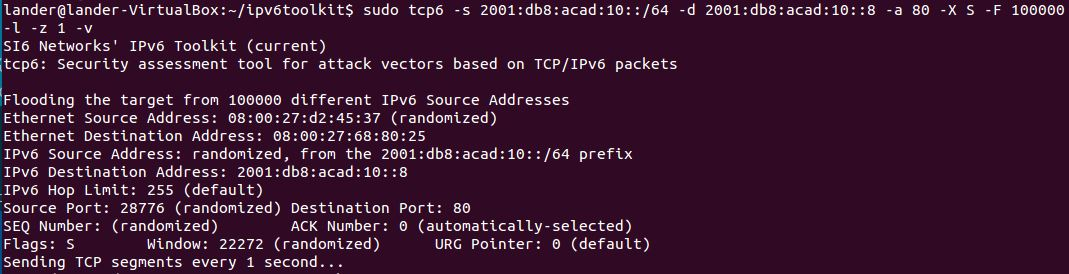
\includegraphics[width=1.0\linewidth]{TCPattack}
  \captionof{figure}{Voorbeeld van een TCP SYN-flood aanval op poortnummer 22 van de host 2001:db8:acad:10::8}
\end{center}


\section{Conclusies}

Het scannen van IPv6-adressen biedt waardevol inzicht in de netwerkstructuur en helpt bij het ontdekken van kwetsbaarheden. Gerichte scans kunnen zwakke punten, zoals open poorten en onveilige configuraties, identificeren. Dit inzicht stelt netwerkbeheerders in staat proactieve maatregelen te nemen om de beveiliging te verbeteren. De Addr6-tool biedt functionaliteit voor het beheer van IPv6-netwerken, zoals het configureren van filterregels en bekijken van gedetailleerde statistieken. De aanval met ICMPv6 error-pakketten kan aanzienlijke schade veroorzaken zonder waarschuwing. Proactieve maatregelen, zoals het configureren van firewalls, verminderen de impact van dergelijke aanvallen. Organisaties moeten zich bewust zijn van de risico's en investeren in robuuste beveiligingsinfrastructuur, regelmatige evaluatie van serverconfiguraties en beveiligingsbewustzijn van medewerkers. Passende beveiligingslagen verminderen de kwetsbaarheid van systemen en waarborgen de netwerkintegriteit. Het onderzoek richt zich op het gebruik van opensource tools voor kosteneffectieve mitigatie van IPv6-aanvallen.

\section{Toekomstig onderzoek}


In de toekomst zal er intensiever onderzoek worden gedaan naar kwetsbaarheden in IPv6, aangezien de adoptie ervan blijft groeien. Dit onderzoek zal zich richten op het ontdekken van nieuwe zwakke punten en het verkennen van opkomende opensource tools voor het beveiligen van IPv6-netwerken. Het is van cruciaal belang om voortdurend te investeren in het bevorderen van onderzoek naar zowel kwetsbaarheden als innovatieve beveiligingstools om de integriteit en vertrouwelijkheid van IPv6-communicatie te waarborgen. Met de toenemende behoefte aan effectieve beveiligingsmaatregelen is het essentieel om proactief te blijven en de nodige maatregelen te nemen om de veiligheid van IPv6-netwerken te waarborgen.

\end{multicols}
\end{document}